\subsection{Experimental Results}
\begin{table*}
\centering
\caption{Experimental results of DCC deployment and high-V\textsubscript{th} assignment}
	\begin{tabular}{l}
	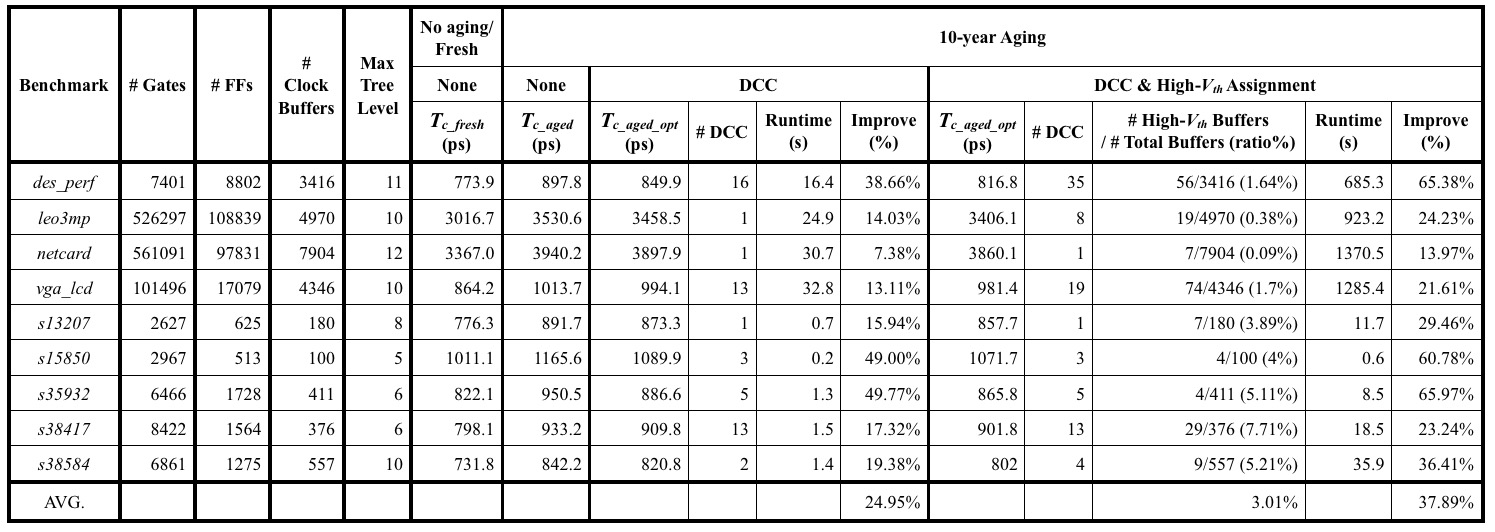
\includegraphics[width=1.7\columnwidth]{Experimental_result_DCC_TVA.png}
	\end{tabular}
\label{table:exp2}
\end{table*}

Table~\ref{table:exp2} shows the experimental results, where Column 4 - 7 demonstrate the former results after applying DCC deployment  and Column 8 - 12 demonstrate the counterparts after applying both DCC deployment and high-V\textsubscript{th} assignment. Column 8 demonstrates the optimum clock period after the two techniques are applied together, denoted by $T_{c\_aged\_opt\_Leader}$. Column 9 demonstrates the used DCC count, Column 10 demonstrates the count of high-V\textsubscript{th} buffers, total count of clock buffers and the ratio of high-V\textsubscript{th} buffers to total clock buffers, and Column 11 demonstrates the run time. The last column demonstrates the improvement, which is the level of aging tolerance and is calculated as:
\begin{gather*}
1 - (T_{c\_aged\_opt\_Leader} - T_{c\_fresh}) / (T_{c\_aged} - T_{c\_fresh})
\end{gather*}
As it can be seen, the proposed framework, which considers the two techniques, can results in lower clock period, implying better improvement for aging tolerance. We can find that, after high-V\textsubscript{th} assignment is included in the former framework, resulting framework may lead to different DCC count. Take \textit{des\_perf} for example, the former DCC count is 7, while the latter DCC count increases to 33. The DCC counts of the two frameworks differ because the DCC deployments are not identical anymore. Specifically speaking, when V\textsubscript{th} assignment is considered, some clock buffers become candidate buffers to be inserted DCC at their inputs, because timing constraints (i.e., setup-time and hold-time) are met based on the inequality Equation (1) and (2), such that DCC can be redeployed to obtain lower Tc. Thus, even thought the two frameworks target the identical benchmark, the DCC deployments/counts may differ. Additionally, the run time of the framework dramatically increases due to numerous possibilities of DCC deployment and leader selection. To be specific, given a pair of flip-flops and associated clock paths, the former framework only considers the possibilities of DCC deployment along the clock paths, while the framework further considers the possibilities of leader selection, for each possibility of DCC deployment. Therefore, the total  possibilities of DCC deployment and leader selection is equal to their mutual multiplication, i.e., DCC possibilities multiplied by leader counterparts, accounting for the dramatic increase of run time.
